
    \documentclass{standalone}
    \usepackage{tikz}
    \usetikzlibrary{arrows, automata, positioning}
    \begin{document}
    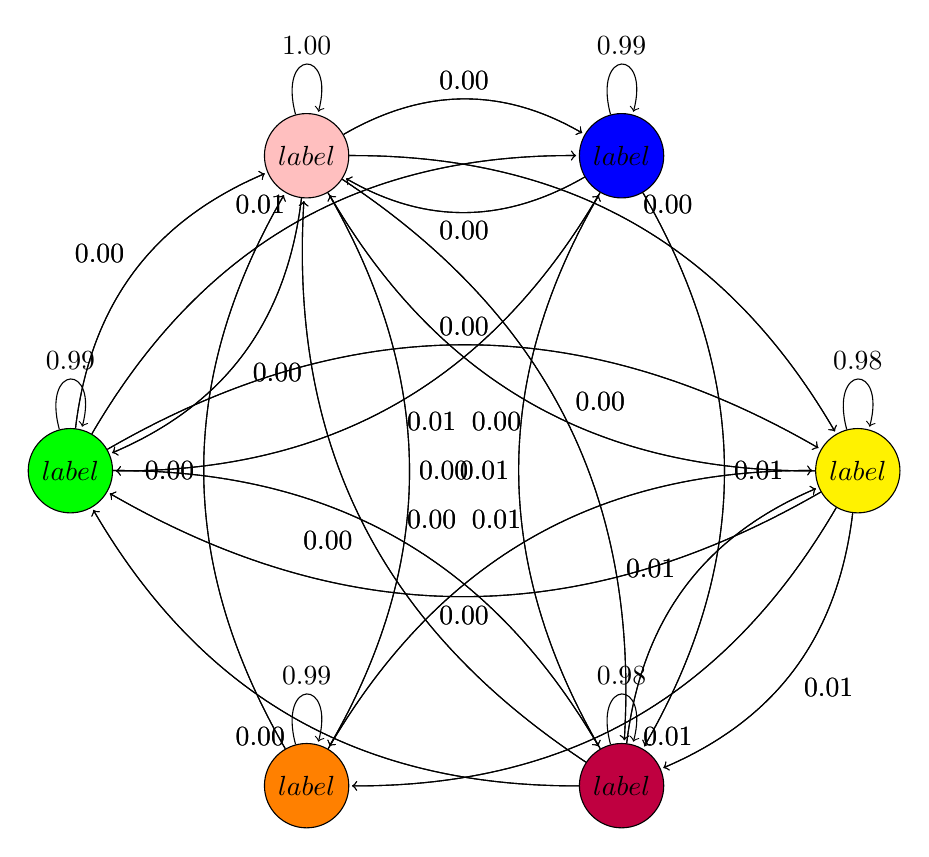
\begin{tikzpicture}[shorten >=1pt, node distance=4cm, on grid, auto]
    \node[state, fill=yellow] (S0) at (5,0) {${label}$} ;
\node[state, fill=blue] (S1) at (2,4) {${label}$} ;
\node[state, fill=pink] (S2) at (-2,4) {${label}$} ;
\node[state, fill=green] (S3) at (-5,0) {${label}$} ;
\node[state, fill=orange] (S4) at (-2,-4) {${label}$} ;
\node[state, fill=purple] (S5) at (2,-4) {${label}$} ;
\path[->] (S0) edge [loop above] node {\(0.98\)} (S0);
\path[->] (S0) edge [bend left] node {\(0.00\)} (S2);
\path[->] (S2) edge [bend left] node {\(0.00\)} (S0);
\path[->] (S0) edge [bend left] node {\(0.00\)} (S3);
\path[->] (S3) edge [bend left] node {\(0.00\)} (S0);
\path[->] (S0) edge [bend left] node {\(0.01\)} (S4);
\path[->] (S4) edge [bend left] node {\(0.01\)} (S0);
\path[->] (S0) edge [bend left] node {\(0.01\)} (S5);
\path[->] (S5) edge [bend left] node {\(0.01\)} (S0);
\path[->] (S1) edge [loop above] node {\(0.99\)} (S1);
\path[->] (S1) edge [bend left] node {\(0.00\)} (S2);
\path[->] (S2) edge [bend left] node {\(0.00\)} (S1);
\path[->] (S1) edge [bend left] node {\(0.01\)} (S3);
\path[->] (S3) edge [bend left] node {\(0.01\)} (S1);
\path[->] (S1) edge [bend left] node {\(0.01\)} (S5);
\path[->] (S5) edge [bend left] node {\(0.01\)} (S1);
\path[->] (S2) edge [bend left] node {\(0.00\)} (S0);
\path[->] (S0) edge [bend left] node {\(0.00\)} (S2);
\path[->] (S2) edge [bend left] node {\(0.00\)} (S1);
\path[->] (S1) edge [bend left] node {\(0.00\)} (S2);
\path[->] (S2) edge [loop above] node {\(1.00\)} (S2);
\path[->] (S2) edge [bend left] node {\(0.00\)} (S3);
\path[->] (S3) edge [bend left] node {\(0.00\)} (S2);
\path[->] (S2) edge [bend left] node {\(0.00\)} (S4);
\path[->] (S4) edge [bend left] node {\(0.00\)} (S2);
\path[->] (S2) edge [bend left] node {\(0.00\)} (S5);
\path[->] (S5) edge [bend left] node {\(0.00\)} (S2);
\path[->] (S3) edge [bend left] node {\(0.00\)} (S0);
\path[->] (S0) edge [bend left] node {\(0.00\)} (S3);
\path[->] (S3) edge [bend left] node {\(0.01\)} (S1);
\path[->] (S1) edge [bend left] node {\(0.01\)} (S3);
\path[->] (S3) edge [bend left] node {\(0.00\)} (S2);
\path[->] (S2) edge [bend left] node {\(0.00\)} (S3);
\path[->] (S3) edge [loop above] node {\(0.99\)} (S3);
\path[->] (S3) edge [bend left] node {\(0.00\)} (S5);
\path[->] (S5) edge [bend left] node {\(0.00\)} (S3);
\path[->] (S4) edge [bend left] node {\(0.01\)} (S0);
\path[->] (S0) edge [bend left] node {\(0.01\)} (S4);
\path[->] (S4) edge [bend left] node {\(0.00\)} (S2);
\path[->] (S2) edge [bend left] node {\(0.00\)} (S4);
\path[->] (S4) edge [loop above] node {\(0.99\)} (S4);
\path[->] (S5) edge [bend left] node {\(0.01\)} (S0);
\path[->] (S0) edge [bend left] node {\(0.01\)} (S5);
\path[->] (S5) edge [bend left] node {\(0.01\)} (S1);
\path[->] (S1) edge [bend left] node {\(0.01\)} (S5);
\path[->] (S5) edge [bend left] node {\(0.00\)} (S2);
\path[->] (S2) edge [bend left] node {\(0.00\)} (S5);
\path[->] (S5) edge [bend left] node {\(0.00\)} (S3);
\path[->] (S3) edge [bend left] node {\(0.00\)} (S5);
\path[->] (S5) edge [loop above] node {\(0.98\)} (S5);

    \end{tikzpicture}
    \end{document}
    